\chapter{Data Distribution}
\label{appendix}
(Referring to the \parencite{GoogleDriveI/O})

The data is synthetically generated by a deep learning model. The data is distributed similarly to the original data that the model was trained on \parencite{ravaghiS04E11MentalHealth2024}.

\resizebox{\textwidth}{!}{ 
\begin{tabular}{|c|c|c|l|}
\hline
 Col\#&  Column name &  datatype&  Feature values\\ 
 \hline
0 & id & int64 &  [0, 1, 2, 3, 4, 5, ...\\ \hline
 1& Name & object & [Aaradhya, Vivan, Yuvraj, ... \\ \hline
 2& Gender & object & [Female, Male] \\ \hline
3 & Age & float64 & [49.0, 26.0, 33.0, ... \\ \hline
4 & City  & object &  [Ludhiana, Varanasi, Visakhapatnam, ...\\ \hline
5 & Working Professional or Student & object & [Working Professional, Student] \\ \hline
6 & Profession & object &  [Chef, Teacher, nan, Business Analyst, ...\\ \hline
7 & Academic Pressure & float64 & [5.0, 4.0, 3.0, 2.0, 1.0] \\ \hline
8 & Work Pressure & float64  &  [5.0, 4.0, 3.0, 2.0, 1.0]\\ \hline
9 & CGPA & float64 & [0-10]  \\ \hline
10 & Study Satisfaction & float64 &  [5.0, 4.0, 3.0, 2.0, 1.0]\\ \hline
11 & Job Satisfaction  & float64 & [5.0, 4.0, 3.0, 2.0, 1.0] \\ \hline
12 & Sleep Duration & object &  [More than 8 hours, Less than 5 hours, 5-6 hours, ...\\ \hline
13 & Dietary Habits & object &  [Healthy, Unhealthy, Moderate, ...\\ \hline
14 & Degree & object & [BHM, LLB, B.Pharm, BBA,... \\ \hline
15 & Have you ever had suicidal thoughts ? &  object &  [No, Yes]\\ \hline
16 & Work/Study Hours & float64  & [1.0, 2.0, ..., 11.0] \\ \hline
17 & Financial Stress & float64 & [5.0, 4.0, 3.0, 2.0, 1.0] \\ \hline
18 & Family History of Mental Illness & object & [No, Yes] \\ \hline
\rowcolor{yellow}
19 & (Target Value) Depression & int64 & [0, 1] \\\hline
\end{tabular}
}

\section{Null Values}

The dataset contains significant missing values for several attributes, including `Profession', `Academic Pressure', `Work Pressure', `CGPA', `Study Satisfaction', `Job Satisfaction', `Dietary Habits', `Degree', and `Financial Stress'.

The missing values can be understood as follows. Students often leave fields such as `Profession', `Work Pressure', and `Job Satisfaction' blank because these attributes are not relevant to their situation, or, in some cases, individuals may not feel comfortable sharing details about their jobs. On the other hand, working professionals tend to omit values for `Academic Pressure', `CGPA', and `Study Satisfaction', as these fields are similarly irrelevant to them.

Other attributes might simply be missing due to the synthetic data generation process. Else, in the case of missing values for `Degree' (two rows), both individuals were identified as working professionals who also chose not to specify their professions. This may suggest discomfort in disclosing qualifications.

The missing values for `Dietary Habits' and `Financial Stress' (four rows each), however, remain unexplained. These omissions do not appear to follow a clear pattern.

\section{Data Analysis} 

As part of the exploratory data analysis (EDA), we plotted the distribution of all features, as well as all features by gender (sensitive attribute) and depression (target). Considering the large number of plots, we only included figures that are essential or surprising in relation to this project in this report. All figures can be found in the Google Colab Notebook. \\

\begin{figure}[H]
    \centering
    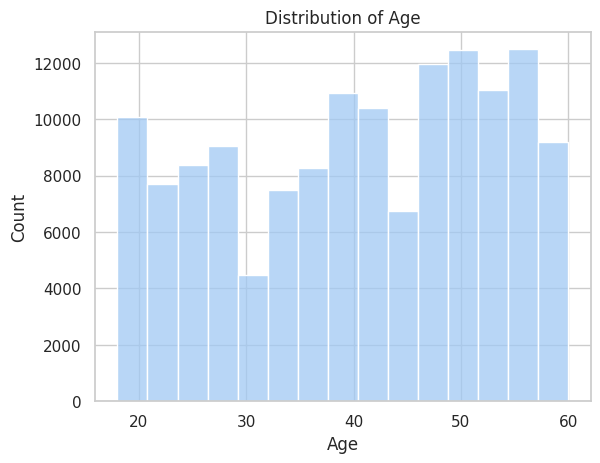
\includegraphics[width=0.5\textwidth]{edafigures/age_dist.png}
    \caption{Distribution of age of the participants.}
    \label{fig:age_dist}
\end{figure}

\noindent Figure~\ref{fig:age_dist} is the general distribution of age of the sample. As you can see, the distribution is approximately uniform, with slightly more older than younger adults.\\

Figure~\ref{fig:gender_dist} is the distribution of gender of the sample. As you can see, there are more males than females in this sample.\\
\begin{figure}[H]
    \centering
    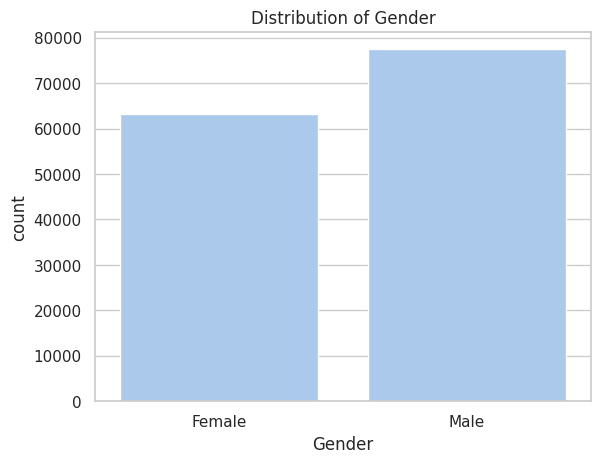
\includegraphics[width=0.5\textwidth]{edafigures/gender_dist.png}
    \caption{Distribution of gender of the participants.}
    \label{fig:gender_dist}
\end{figure}
Similarly, the distribution of depression is presented as figure~\ref{fig:dep_dist}. Not surprisingly, the rate of depression is relatively low, which is consistent with our expectation. However, the prevalence of depressed individuals in this sample is 18.2\%, which is way higher than the population average. Considering the data is synthetically generated with the purpose of depression detection, the depression prevalence can be explained. 

\begin{figure}[H]
    \centering
    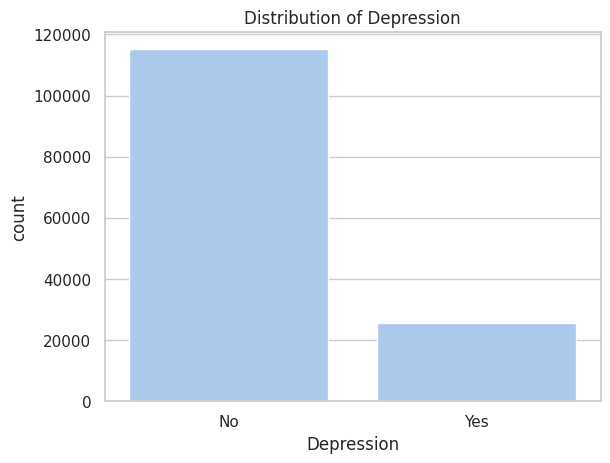
\includegraphics[width=0.5\textwidth]{edafigures/dep_dist.png}
    \caption{Distribution of depression.}
    \label{fig:dep_dist}
\end{figure}

To get a basic sense of how depression distributes relative to our sensitive attribute, gender, we plotted depression by gender. The resulting figure is figure~\ref{fig:dep_gender}. Contrary to our expectation and general consensus \parencite{APA2013DSM5}, there are slightly more depressed males than there are females. One potential explanation is that the data is simulating features of Indian population, which could have a different gender prevalence when it comes to depression than the one based on almost completely U.S. and Western context. \\

\begin{figure}[H]
    \centering
    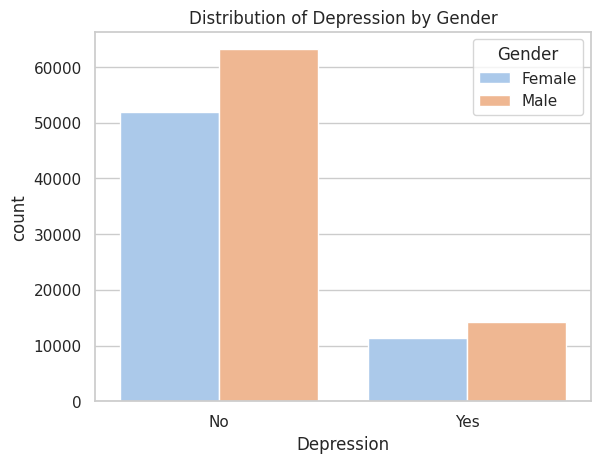
\includegraphics[width=0.6\linewidth]{edafigures/dep_gender.png}
    \caption{Depression by Gender.}
    \label{fig:dep_gender}
\end{figure}

Another interesting aspect of this dataset we discovered through EDA is the distribution of age in terms of depression. See figure~\ref{fig:age_dep}. The mean age of depressed individuals is substantially lower than that of the not depressed ones, at around 23 years of age, while the mean age of not depressed participants is around 35. The age distribution aligns with published studies on the age of onset of depression \parencite{mirowskyAgeDepression1992}, where there is a large spike in depression rate for people between the ages of 17 and 25, and again for people that are over 80 years of age. Though there are more working professionals than students in this dataset (results not shown), there is a much higher rate of depression in young adults. This trend indicates a possibility of treating age as a sensitive attribute, as it might lead to imbalanced model prediction based on age alone. To explore this possibility, we calculated the point-biserial correlation of age and depression, which we will present and report in the later sections. 
\begin{figure}[H]
    \centering
    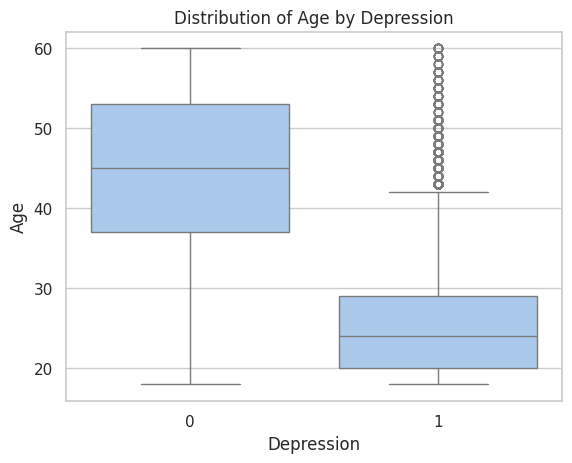
\includegraphics[width=0.6\linewidth]{edafigures/age_dep.png}
    \caption{Distribution of age by depression.}
    \label{fig:age_dep}
\end{figure}

\begin{figure}[H]
    \centering
    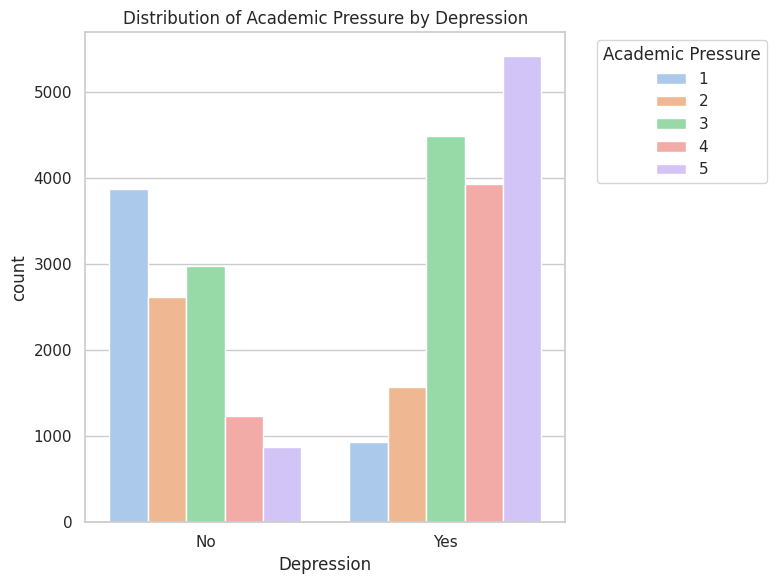
\includegraphics[width=0.6\linewidth]{edafigures/academicPressure_dep.png}
    \caption{Distribution of academic pressure and depression.}
    \label{fig:academicPressure_dep}
\end{figure}

Figure~\ref{fig:academicPressure_dep} illustrates the relationship between academic pressure and depression. The distribution for non-depressed individual is clearly negatively skewed, while the distribution for depressed individual is the direct opposite. This result makes intuitive sense, as one would expect the perceived stress would have a relationship with depression. Similar trends are observed in the relationship between work pressure and depression, and opposite trends are observed in the relationship between study satisfaction and job satisfaction and depression, in the sense that depressed individuals reported less satisfaction in their study or job than non-depressed individuals.

% \newpage
\subsection{Feature Correlation}\label{feature_corr}

As illustrated in Figure~\ref{fig:age_dep}, the sigmoid curve depicted in Figure~\ref{fig:prob_age_depression} clearly demonstrates that the probability of depression is higher among young adults. This can be attributed to the fact that students exhibit significantly higher rates of depression compared to working professionals (Figure~\ref{fig:depression_empoyment}). Furthermore, the correlation matrix shown in Figure~\ref{fig:corr_depression} emphasizes that attributes such as unhealthy dietary habits, inadequate sleep duration, and the occurrence of suicidal thoughts are positively correlated with each other and are notably associated with students. 

\begin{figure}[H]
    \centering
    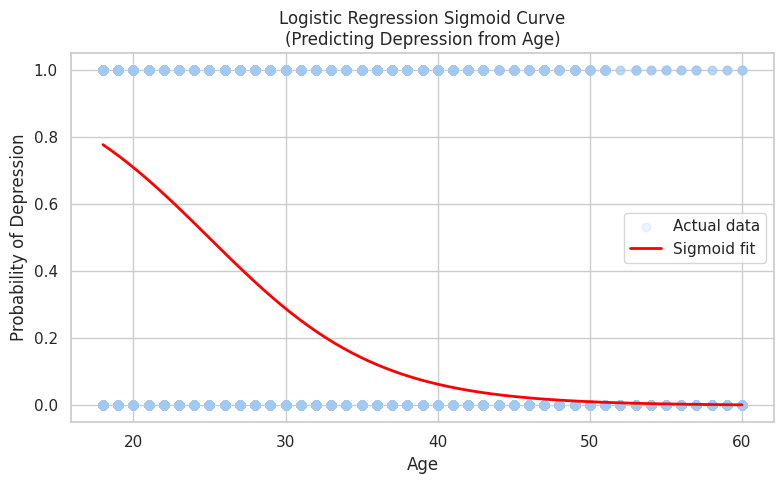
\includegraphics[width=0.5\linewidth]{edafigures/prob_age_depression.png}
    \caption{Predicting Depression from Age}
    \label{fig:prob_age_depression}
\end{figure}

\begin{figure}[H]
    \centering
    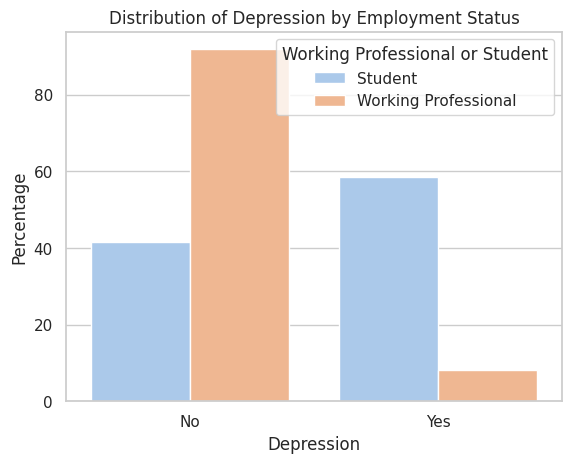
\includegraphics[width=0.5\linewidth]{edafigures/depression_empoyment.png}
    \caption{Distribution of Employment Status vs Depression}
    \label{fig:depression_empoyment}
    
\end{figure}

\begin{figure}[H]
    \begin{minipage}{0.5\textwidth}
        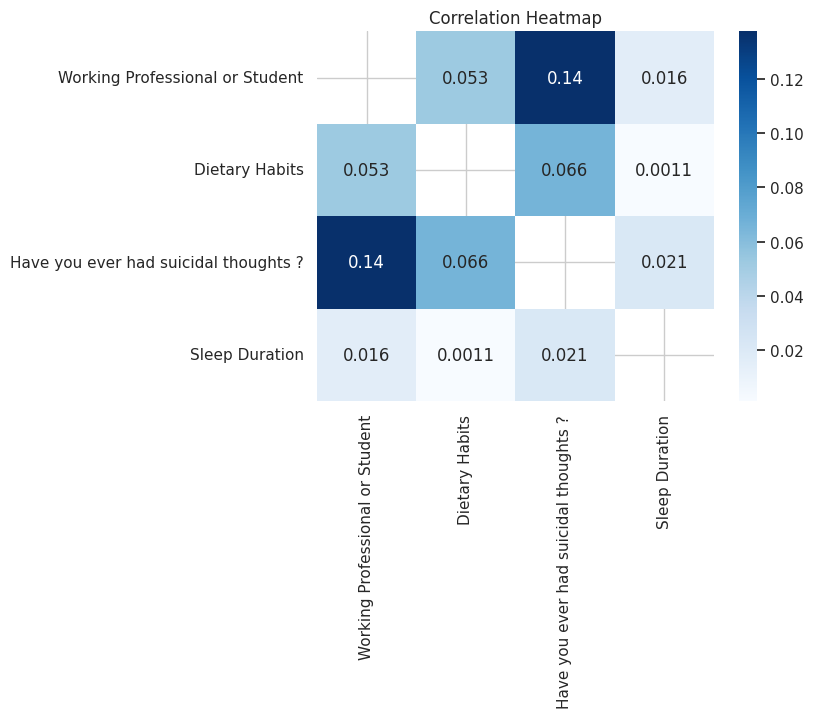
\includegraphics[width=\linewidth]{edafigures/corr_depression.png} 
        \caption{Correlation of Employment Status, Dietary Habits, Sleep Duration and Suicidal Thoughts.}
    \label{fig:corr_depression}
    \end{minipage}
    \hfill
    \begin{minipage}{0.45\textwidth}
        \scriptsize{
        Student:1, Working Professional:0\\
        Unhealthy: 2, Moderate: 1, Healthy:0\\
        Sleep : $<$ 5 hours:3, 5-6 hours:2, $>$ 8 hours: 1, 7-8 hours: 0\\
        Suicidal Thoughts: Yes: 1, No: 0}
    \end{minipage}
\end{figure}

Our analysis as shown in Figure~\ref{fig:corr_gender_work} also reveals a positive correlation between gender (-1 for males, 1 for females) and work pressure, consistent with prior studies indicating women face higher work pressure due to overlapping professional and caregiving roles, especially during remote work setups \parencite{rabuni2023worklifebalance}.

\begin{figure}[H]
    \centering
    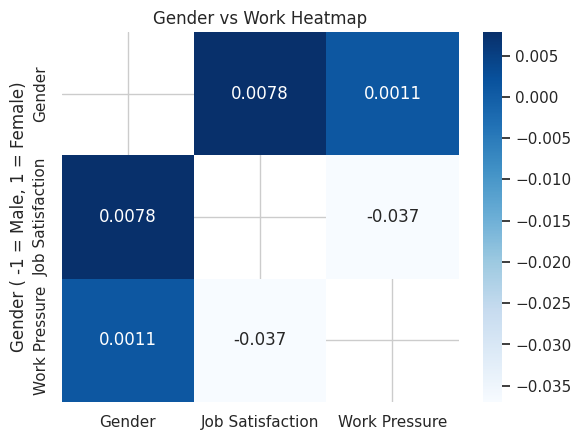
\includegraphics[width=0.5\linewidth]{edafigures/corr_gender_work.png}
    \caption{Distribution of Gender vs Work Pressure and Job Satisfaction}
    \label{fig:corr_gender_work}
\end{figure}

Interestingly, the data also indicates a positive correlation between gender and job satisfaction. This observation appears to contradict prior studies that associate lower job satisfaction among women with discriminatory organizational practices and societal expectations \parencite{karthikkumar2024worklifebalanc}. One potential explanation for this contradiction might lie in the study's context—data was collected from selected urban cities in India, where unique factors could influence these findings. For instance, exceptions in prior research suggest that variables such as locus of control can sometimes neutralize gender disparities in job satisfaction \parencite{talamala2024locuscontrol}.


Another aspect of the data distribution is shown in Figure~\ref{fig:regionwise} and~\ref{fig:regional_distri} , which suggests that dataset primarily includes data from major cities in larger states of India, predominantly from the Central North and Central-West regions. This lack of data from small-to-medium cities, rural areas, and regions like the South, Central-East, and North-East India might be an unrepresentative sample.
\begin{figure}[H]
    \centering
    \begin{minipage}{0.45\textwidth}
        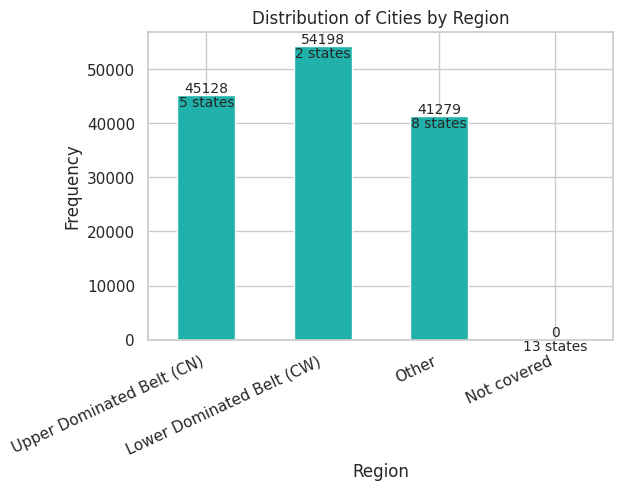
\includegraphics[width=\linewidth]{edafigures/regionwise.png}
        \caption{Data Distribution Region-wise}
        \label{fig:regionwise}
    \end{minipage}
    \hfill
    \begin{minipage}{0.45\textwidth}
        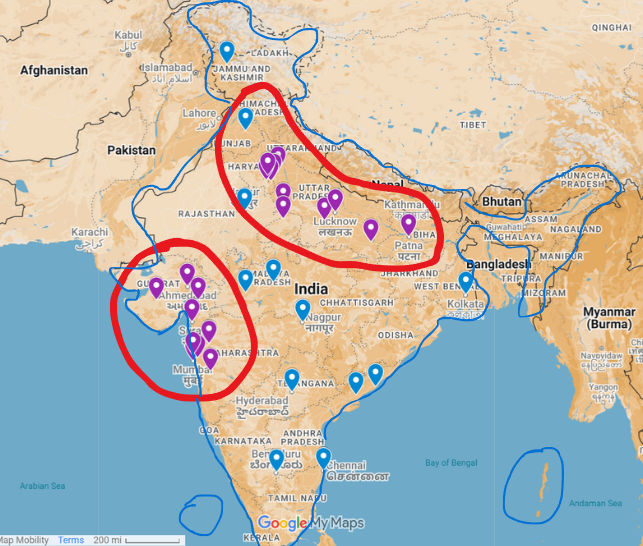
\includegraphics[width=\linewidth]{edafigures/regional_distri.png}
        \caption{Map Annotation of Training Data, depicting biased selection}
        \label{fig:regional_distri}
    \end{minipage}
\end{figure}

\section{Post Training Analysis}\label{post_train}

\begin{figure}[h]
    \centering
    
\includegraphics[width=0.6\linewidth]{figures/regionwise.png}
    \caption{Overall Performance w.r.t. Region After Model Training}
    \label{fig:region_overall}
\end{figure}

\begin{figure}[H]
    \centering
    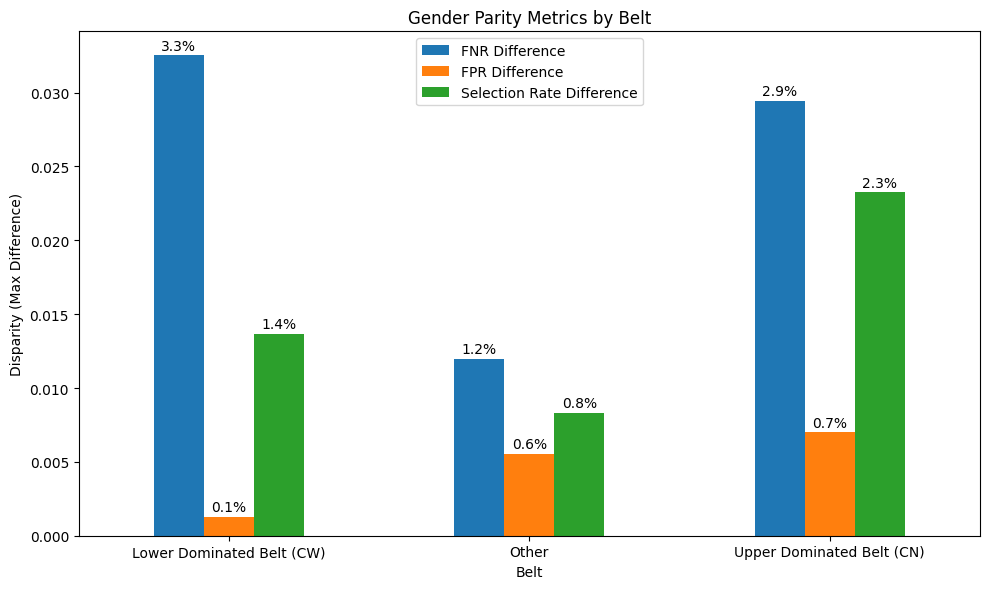
\includegraphics[width=0.6\linewidth]{figures/region_parity.png}
    \caption{Fairness w.r.t. Gender for Region After Model Training}
    \label{fig:region_gender}
\end{figure}

\begin{figure}[H]
    \centering
    \begin{minipage}{0.48\textwidth}
            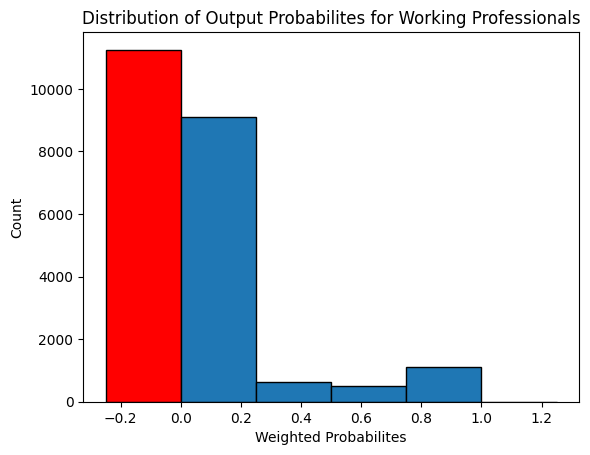
\includegraphics[width=\linewidth]{figures/prob_distri_prof.png}
    \end{minipage}
    \hfill
    \begin{minipage}{0.48\textwidth}
         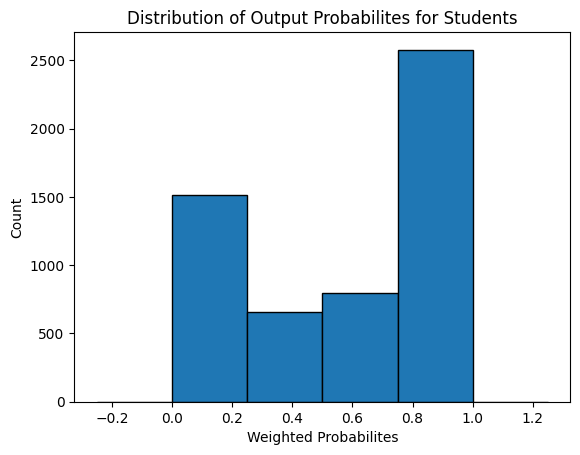
\includegraphics[width=\linewidth]{figures/prob_distri_stu.png}
    \end{minipage}
    \caption{The output ``probabilites" for Working Professionals are outside the range of [0,1], with a significant count in less than 0, which cannot be ignored or considered outliers. This imply that there is an in-processing need for scaling such distribution, as they don't clearly justify the predicted outcome. This also strengthens the argument for optimizing threshold for classification.}
    \label{fig:prob_distri}
\end{figure}


